\chapter{Design}\label{chapter:design} \

In Section~\ref{section:datasets} from Chapter~\ref{chapter:design} 
we will introduce the chosen datasets (as well as the
preprocessing applied on them) to be used in the experiments.
Additionally, in Section~\ref{section:state_preparation_noise}
we will present the design decisions taken when implementing
noisy coherent \ac{qml} models due to the impact of
state preparation noise. \

\section{Datasets}\label{section:datasets} \

In this section we will present which datasets are used in the thesis
and the reasons why they were included. Current capabilities of
quantum computers do not allow for big and complex quantum circuits
to be executed. Thus, most of the datasets will have a smaller
feature set in comparison to datasets used to benchmark classical
\ac{ml} models. \

The dataset selection was heavily influenced by the datasets utilized in
~\cite{winderl_quantum_2023}. All the datasets but the Plus-Minus
Dataset were retrieved from OpenML~\cite{vanschoren_openml_2014} using
Scikit-learn~\cite{pedregosa_scikit-learn_2011} in Python. All data
points that had missing features were removed, as well as all duplicate
data points. Finally, all the datasets (except the Iris Flower Dataset
~\ref{subsection:iris}) have been normalized per feature using the
standard deviation and the resulting values were rescaled into the
range between  [0,1]. \

\subsection{Iris Flower Dataset}\label{subsection:iris} \

The Iris Flower Dataset~\cite{fisher_use_1936} is a collection of
150 data points regarding three different species of the Iris flower.
Four features were collected, namely the length and width of the sepals
and petals. For this dataset we made a special adaptation such that
we would replicate the dataset used by~\cite{du_quantum_2021}. This
adjustment is removing all data points with the class label
\textit{virginica} and setting the feature \textit{petal width}
to \(0\). \

\begin{figure}[h!]
  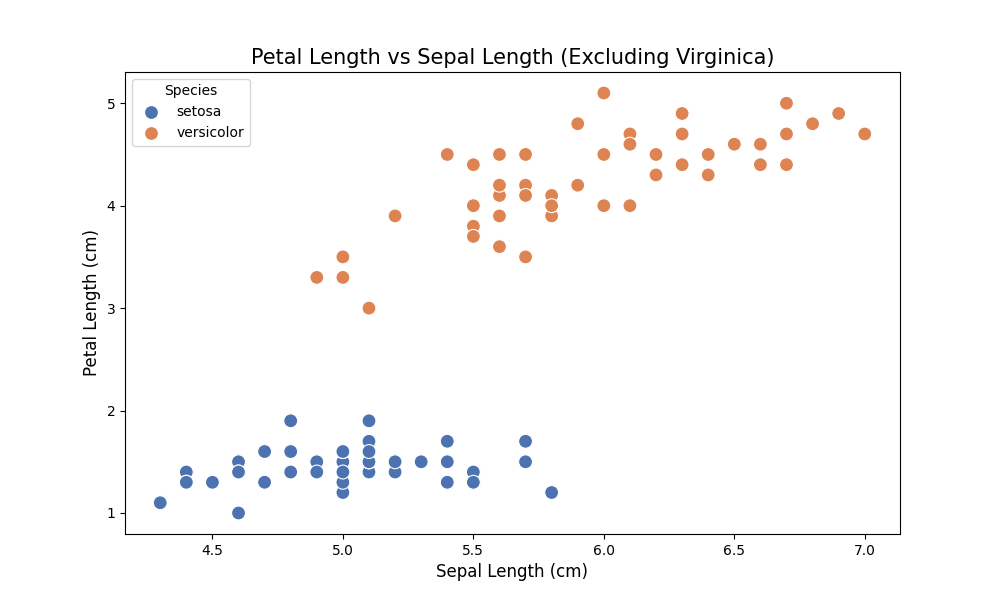
\includegraphics[scale=0.5]{figures/iris-linear-separation.png}
  \centering
  \caption{Data plot of the Iris dataset's \textit{Sepal Length} and \textit{Sepal Length} features.}
~\label{fig:iris_linear}
\end{figure} \

In Figure~\ref{fig:iris_linear} we can observe the purpose of these
modifications. By removing the \textit{virginica} class we can
linearly separate the dataset by using two different features,
e.g.\ the \textit{petal length} and \textit{sepal length}. Furthermore,
removing the feature \textit{petal width} makes the model focus on
the other features, eliminating overhead and ensuring the \ac{qml}
will converge to an optimal solution quicker. \

\subsection{Pima Indians Diabetes Dataset}\label{subsection:diabetes} \

The \ac{pid} Dataset~\cite{smith_using_1988} contains
768 data points collecting 8 features that were considered risk
factors for the onset of diabetes. This dataset presents a class
imbalance. To remediate the asymmetry in the classes distribution
we removed 232 data points from the \textit{negative} class. The
removal was performed randomly with a fixed seed to always
keep the same data points and make the results reproducible. \

A class imbalance can lead to reduced performance of a \ac{ml} model
~\cite{drummond_c45_nodate}. This decrease in accuracy could
probably be translated to \ac{qml} models as well. Therefore,
with the removal of the data points from the majority class, we
obtain a completely balanced dataset and model performance should
be maximized. \

\pagebreak

\subsection{Wisconsin Breast Cancer (Diagnostic) Dataset} \

The Wisconsin Breast Cancer Dataset~\cite{street_nuclear_1993} is
composed by 699 data points collecting 10 features of breast masses
that could potentially be carcinogenic. While this set is also
unbalanced as the original \ac{pid} Dataset~\ref{subsection:diabetes},
the asymmetry is not as pronounced. We left the class distribution
untouched to check whether the \ac{qml} models would overcome class
distribution imbalance. \

It is interesting to note that in~\cite{winderl_quantum_2023}
they reported that normalizing the dataset per feature with the
standard deviation hindered the convergence of the \ac{qml} models.
However, we didn't experience this when training our \ac{qml} models,
thus, we do normalize the data with the standard deviation per feature. \

\subsection{Plus-Minus Dataset}\label{subsection:plus-minus} \

The Plus-Minus Dataset~\cite{wendlinger_comparative_2024} is made of
1,200 grayscale images, each containing \(18 \times 18 = 324\) pixels.
Inside each image we can observe four different classes, respectively
the symbols \(-\), \(+\), \(\vdash\) and \(\dashv\). By utilizing this
dataset, we will be able to interpret the perturbations caused by
the adversarial attacks better. For example, if an adversarial attack
trying to force the \ac{ml} model into misclassifying \(\vdash\) into
a \(+\), the most obvious semantical modification would be to add an
horizontal line. \

In~\cite{west_benchmarking_2023}, they observed that \ac{qml} models
focus on different more robust features in the input data than
\ac{ml} models. This dataset will help us verify this claim and
provide deeper insight into the semantic meaning of adversarial
attacks, specifically in the quantum setting. \

\subsection{MNIST Dataset}\label{subsection:mnist} \

The MNIST Dataset~\cite{bottou_comparison_1994} is composed by
70,000 images representing handwritten individual digits between
the range from \(0\) to \(9\). Each image is a monocromatic gray scale
image shaped by \(28 \times 28 = 746\) pixels. A \ac{qml} model would
require 10 qubits to encode the features with the amplitude embedding
technique. Because the amount of operations required for the
\ac{qml} model to process the data increments exponentially, the model
quickly becomes intractable to train in commonly available hardware.
Therefore, we downsample the images by half to \(16 \times 16 = 256\) and
the \ac{qml} model would now only require 8 qubits. In Figure
~\ref{fig:mnist_resized} we can observe that downsampling the images
does not significatively visually affect the image recognition. \

\begin{figure}
  \centering
  \begin{subfigure}{0.35\textwidth}
    \centering
    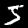
\includegraphics[width = \textwidth]{figures/reshaped.jpg}
    \caption{Original image.}
  \end{subfigure} \qquad \qquad
  \begin{subfigure}{0.35\textwidth}
    \centering
    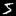
\includegraphics[width = \textwidth]{figures/resized.jpg}
    \caption{Downsampled image.}
  \end{subfigure}
  \caption{Visual comparison between both images.}\label{fig:mnist_resized}
\end{figure} \

Similar to~\cite{lu_quantum_2020} we further divide the MNIST
set to simulate a binary classifier and a 4-class classifier task. The
resulting datasets are named MNIST2 and MNIST4 respectively. To obtain
the MNIST2 dataset, we exclude all classes but the images that contain
a one or a nine. Furthermore, to retrieve the MNIST4 dataset we kept
all the images with digits one, three, seven and nine. With this extension
we can now compare how the \ac{qml} models accuracy varies with the
amount of classes to categorize. \

\section{State Preparation with Coherent Noise}\label{section:state_preparation_noise} \

In the next chapter (Sec.~\ref{section:vqa_training}) the trained variational circuit classifiers
utilize the amplitude embedding technique to encode classical data
into the \ac{qml} model. Pennylanes's \colorbox{inline_gray}{\lstinline|AmplitudeEmbedding|}~\cite{bergholm_pennylane_2022}
is utilized to encode the data accordingly. In this subsection we will
present the impact of state preparation with coherent noise on quantum
circuits. \

In order to simulate coherent noise we used Qiskit's Aer noise simulator.
Qiskit's noise models can be linked with Pennylane by declaring them as
an argument when creating a device. We attach coherent noise per gate
with the noise's corresponding unitary matrix. The unitary matrices are
derived with their respective rotational matrices \(R_{Y}\), \(R_{Z}\) and 
\(CR_{X}\) with a small \(\theta = \epsilon\). In this case we set 
\(\epsilon\) to be around 0.175 to simulate a \(10^{\circ}\) gate
miscalibration. \

The test circuits are composed first by an
\colorbox{inline_gray}{\lstinline|AmplitudeEmbedding|} state preparation
layer. Then, a single quantum gate follows that will characterize the
test circuit. In total there are three test circuits that describe the
effect of coherent noise on the \(R_{Y}\), \(R_{Z}\) and \ac{cnot} gates.
These gates were chosen because they are utilized by the strongly
entangling layers ansatz. For the rotational gates, a \(\theta = \pi\)
angle was chosen to simulate their equivalent non-rotational gates. \

In Table~\ref{tab:ry_noise} we can observe the ideal noiseless results
for the \(R_{Y}(\pi)\) gate in the third column. This table yields the
same result as applying the Pauli Y gate. We use the Pauli Z matrix as
the observable. The projective measurement values will be between the
range of -1 and 1. \

\begin{table}[h]
  \centering
  \begin{tabular}{|c|c|c|c|c|}
    \hline
    Quantum State & \(R_{Y}\left(\pi\right)\) & \(\expval{Z}\) & Expected \(R_{Y}\left(\pi+\epsilon\right)\) & Obtained \(R_{Y}\left(\pi+\epsilon\right)\) \\
    \hline
    \(\ket{0}\) & \(i\ket{1}\)  & -1 & -0.985 & -0.985 \\
    \hline
    \(\ket{1}\) & \(-i\ket{0}\) &  1 &  0.985 &  0.940 \\
    \hline
    \(\ket{+}\) & \(-i\ket{-}\) &  0 &  0.174 &  0.340 \\
    \hline
  \end{tabular}
  \caption{Expectation value with Pauli Z observable of \(R_{Y}\) gate with \(\theta = \pi\) and \(\epsilon = 10^{\circ}\).
  The fourth column represents the calculated effects of coherent noise without state preparation.
  The fifth column represents the results of coherent noise with state preparation and Qiskit's Aer device.}\label{tab:ry_noise}
\end{table} \

The calculated expectation values for the \(R_{Y}(\theta + \epsilon)\) gate
can be found in the fourth column of Table~\ref{tab:ry_noise}. We can
observe that the measurements from the resulting quantum state are
perturbed. For the computational basis states the expected value is
equally reduced in magnitude. For the superposition state \(\ket{+}\),
the expected value 0 is shifted by the coherent noise. The magnitude
of the disturbances from the measurements is directly proportional to
\(\epsilon\) up to a phase of \(2\pi\). \

The experimental results from adding coherent noise to the
\(R_{Y}(\theta)\) gate are presented in the fifth column of Table~\ref{tab:ry_noise}. 
While for the \(\ket{0}\) state the result does match the calculated
-0.985 value, for the other two tested quantum states there is a
notable difference between the calculated and the experimental results. \

In relation to the test from the \(R_{Z}(\theta + \epsilon)\) gate, we
are not able to observe any effect of either the rotation or the noise.
This is because any Z transformation only modifies the phase of the
quantum state, which cannot be measured with the Pauli Z observable.
However, it is important to note that in the experimental results
a difference of around 0.001 was observed in the result of the \(\ket{+}\)
state measurement. \

For the \ac{cnot} gate circuit we tested both cases (a control qubit on the
first wire and a target qubit on the second wire and vice versa). For
the first case of the \ac{cnot}  gate circuit test, the noiseless expectation
values with the Pauli Z observable can be found in the third column of Table
~\ref{tab:cnot_noise}. Similarly to the \(R_{Y}(\theta)\) circuit test,
the expectation values lie between a range of -1 and 1. Contrarily,
for the case of the \ac{cnot}  gate we measure at the end of the circuit the
two qubits from the quantum state. \

\begin{table}[h]
  \centering
  \begin{tabular}{|c|c|c|c|c|}
    \hline
    Quantum State & \ac{cnot} & \(\expval{Z}\) & Expected \(\expval{Z}+\epsilon\) & Obtained \(\expval{Z}+\epsilon\) \\
    \hline
    \(\ket{00}\) & \(\ket{00}\) & [1, 1]   & [1, 1]       & [1, 1]          \\
    \hline
    \(\ket{01}\) & \(\ket{01}\) & [1, -1]  & [1, -1]      & [0.992, -0.996] \\
    \hline
    \(\ket{10}\) & \(\ket{11}\) & [-1, -1] & [-1, -0.985] & [-0.985, -1]    \\
    \hline
    \(\ket{11}\) & \(\ket{10}\) & [-1, 1]  & [-1, 0.985]  & [-0.992, 0.996] \\
    \hline
  \end{tabular}
  \caption{Expectation value with Pauli Z observable of \ac{cnot} gate with \(\epsilon = 10^{\circ}\).
  The fourth column represents the calculated effects of coherent noise without state preparation.
  The fifth column represents the results of coherent noise with state preparation and Qiskit's Aer device.}\label{tab:cnot_noise}
\end{table} \

In Table~\ref{tab:cnot_noise} we can find in the fourth column the calculated
projective measurements with the Pauli Z matrix for the \ac{cnot} gate.
First of all we can observe that for the quantum states \(\ket{00}\)
and \(\ket{01}\) the values don't incur in any noise as the control
qubit is set to 0 and the Pauli X rotation is not performed on the target
qubit. Notwithstanding, for \(\ket{10}\) and \(\ket{11}\), where the
control qubit is set, noise should be present in the second qubit's
measurements with an equal magnitude. \

The experimental results from adding coherent noise to the
\ac{cnot} gate are presented in the fifth column of Table~\ref{tab:cnot_noise}.
Although the result for the \(\ket{00}\) state is the same as the
previously calculated value, the experimental values obtained for
the other three states differ. For the \(\ket{01}\) state there
should be no noise present, however, both qubit measurements
show disturbances in their value. Regarding the \(\ket{10}\) state
the measurement values for both qubits are inverted. Finally,
for the \(\ket{11}\) state the first qubit shows signs of noise
when it should not, while the second qubit exhibits a different noise
magnitude than calculated. \

In theory the effects of coherent noise should be deterministic,
as their effects can be described by a unitary matrix applied
every time once a gate has been executed. In spite of that,
the observed results from the experimental tests indicate that
coherent noise with Qiskit's noise models plugged into Pennylane
are not deterministic and fluctuate between a small margin range. \

All the gates that we tested presented differences with the
calculated and obtained results. After further investigation
we determined that the additional noise arises from the state
preparation routine. In Pennylane's documentation we found that
the \colorbox{inline_gray}{\lstinline|AmplitudeEmbedding|} function
inherits from the \colorbox{inline_gray}{\lstinline|StatePrep|}
function. Furthermore, there is a note that indicates
if \colorbox{inline_gray}{\lstinline|StatePrep|} is not supported
by the device, the method developped by Möttönen et al.~\cite{mottonen_transformation_2004}
will be utilized. \

The state preparation method proposed by Möttönen et al.\ utilizes a
combination of \(R_{Y}(\theta)\), \(R_{Z}(\theta)\) and \ac{cnot}
gates to transform a quantum state \(\ket{a}\) into another quantum state
\(\ket{b}\). For \(n\) qubits this method has an upper bound of
\(2^{n+2}-4n-4\) \ac{cnot} gates and \(2^{n+2}-5\) one-qubit elementary
rotation gates (both \(R_{Y}(\theta)\) and \(R_{Z}(\theta)\)). These
bounds grow exponentially, therefore their impact in conjunction with
quantum noise will be greatly augmented with the number of qubits used.
On the other hand, the bounds can be halved for special cases, e.g.\ when
the initial or the final quantum state is a basis vector. \

We performed some tests to see the impact state preparation has on
a quantum circuit running on Qiskit's Aer noise simulator. The experiment
consists on transforming the initial quantum state \(\ket{0_{n}}\)
(where \(n\) is the number of qubits) to the quantum state where the
magnitude of all the possible amplitude probabilities is equal. \

\begin{figure}[h!]
  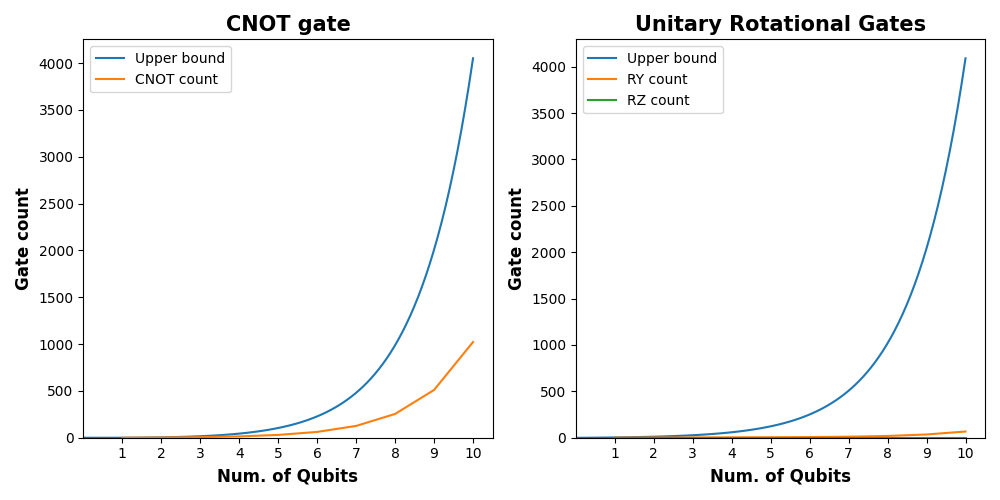
\includegraphics[scale=0.55]{figures/state-prep-gates-count.png}
  \centering
  \caption{Observed required gates to perform state preparation with Möttönen's method.}
~\label{fig:state_prep}
\end{figure} \

In Figure~\ref{fig:state_prep} the theoretical upper bounds of
Möttönen's state preparation method for both types of gates can
be distinguished from the obtained gate counts in the experiment.
While we can experimentally appreciate that the actual gate count
does not grow as fast as the theoretical upper bounds (mainly because
of the special case where we start from a computational basis vector),
we can still observe an exponential growth in the \ac{cnot} gate count.
Thus, if we perform state preparation with Möttönen's method, it will
represent a significant source of noise impacting the \ac{qml} model. \

To better comprehend the previously obtained coherent noise experimental
results we created an artificial coherent noise simulation. This
simulation utilizes Pennylane's \colorbox{inline_gray}{\lstinline|default.qubit|}
device, which does not incur in any type of noise. To artificially
introduce coherent noise into the quantum circuit we extract the
performed quantum gates Möttönen's method would use for state
preparation and after each gate introduce a corresponding rotational
gate with \(theta = \epsilon\). \

The results of the artificial coherent noise \ac{cnot} gate test are found
in Table~\ref{tab:cnot_artificial_noise}. Although they still don't
match the calculated ideal measurements from Table~\ref{tab:cnot_noise},
we can attribute the differences to noise incurred during state preparation
using Möttönen's method. There should be no noise in any first qubit
measurement, however, for the quantum states \(\ket{10}\) and \(\ket{11}\)
state preparation for the first qubit causes noise in the measurements.
Regarding the second qubit measurements, \(\ket{10}\) and \(\ket{11}\)
should show less signs of noise. For \(\ket{01}\), there should not be
any incurred noise. Again, the differences can be attributed to noise
sustained during noise preparation. \

\begin{table}[h]
  \centering
  \begin{tabular}{|c|c|c|}
    \hline
    Quantum State & \(\expval{Z}\) \\
    \hline
    \(\ket{00}\) & [1, 1] \\
    \hline
    \(\ket{01}\) & [1, -0.940] \\
    \hline
    \(\ket{10}\) & [-0.985, -0.852] \\
    \hline
    \(\ket{11}\) & [-0.985, 0.929] \\
    \hline
  \end{tabular}
  \caption{Obtained artificial expectation value with Pauli Z observable of \ac{cnot} gate with \(\epsilon = 10^{\circ}\).
  The results include coherent noise induced by state preparation. }\label{tab:cnot_artificial_noise}
\end{table} \

We can look into a specific case to further specify the influence
of coherent noise during state preparation. In Equation
~\ref{eq:cnot_artificial} the quantum circuit describing the state
preparation using Möttönen's method and then applying one \ac{cnot} gate
is illustrated. The state preparation part from the quantum circuit is
enclosed by a dotted line box. The initial quantum state is \(\ket{00}\)
and it is being transformed into \(\ket{01}\) by utilizing two
\(R_{Y}(\theta)\) and two \ac*{cnot} gates. We can observe that after
each operation there is a rotational gate that correspond to the coherent
noise. \

\begin{equation}\label{eq:cnot_artificial}
  \Qcircuit @C=0.4em @R=0.4em {
    & \qw                         & \qw                    & \ctrl{1} & \ctrl{1}               & \qw                         & \qw                    & \ctrl{1} & \ctrl{1}               & \ctrl{1} & \ctrl{1}               & \meterB{Z} \\
    & \gate{R_{Y}(\frac{\pi}{4})} & \gate{R_{Y}(\epsilon)} & \targ    & \gate{R_{X}(\epsilon)} & \gate{R_{Y}(\frac{\pi}{4})} & \gate{R_{Y}(\epsilon)} & \targ    & \gate{R_{X}(\epsilon)} & \targ    & \gate{R_{X}(\epsilon)} & \meterB{Z}
    \gategroup{1}{1}{2}{9}{0.8em}{--}
  }
\end{equation} \

In this specific case, because the control qubit is set to 0, none
of the control gates will perform any modification to the target wire.
The control gates also don't modify the control qubit, thus, there are
no perturbations in the measurement. Furthermore, we can simplify
all the \(R_{Y}(\theta)\) gates into one by adding up their angles. The
resulting gate is then \(R_{Y}(\frac{\pi}{2}+2\epsilon)\). If we 
then apply the gate, we obtain the quantum state \(\ket{\psi} =
R_{Y}(\frac{\pi}{2}+2\epsilon)\ket{0}\). We can now calculate
the expectation value \(\expval{Z}{\psi}\) and the result will
be -0.940 for an \(\epsilon = 0.175\), which is exactly what we get
as a result in Table~\ref{tab:cnot_artificial_noise}. \

One important conclusion regarding this experiment is that the
quantum state \(\ket{0}\) does not require to be modified during
the state preparation routine, consequently, it will not display
any coherent noise disturbance. In addition, any control gate will
not introduce any coherent noise to the target qubit if the control
qubit is set to 0. \

Finally, in the artificial test we get deterministic measurements that
better represent coherent noise. Hence, for any further experiment
utilizing coherent noise, we will combine Pennylane's
\colorbox{inline_gray}{\lstinline|default.qubit|} with corresponding
rotational gates after each quantum gate to achieve a model closer
to reality. \

% TODO: Think if using classical AML makes sense (west_benchmarking_2023)
%       - probably not, paper says QVC are resilient to classical attacks
%       - maybe train one classical model, perform attack and check how the QVC behaves

% FOCUS ON QAML (MAYBE DO CLASSICAL TRANSFER ATTACKS)

% Maxi says not all qml models are robust to transfer attacks from classical ml / Amplitude encoding works differently (focuses on several areas of the image)

% MENTION AMPLITUDE ENCODING DIFFERENT BEHAVIOUR (MAYBE: DO MORE ENCODING TYPES)

% TODO: Think which comparisons are going to be made: (check transferability between models)
%       - QAML without any noise: Test on vanilla and noise induced QML models
%       - QAML with noise: Test on vanilla and noise induced QML models

% FOCUS ON THE FULL NOISE AND BASELINE NO NOISE (MAYBE DO COMBINATIONS AFTERWARDS)

% TODO: How to perform QAML? How to transform aml attacks into qaml?
%       - Find unitary similar to identity and disturb input quantumm state? (qaml) (parameters 2^n x 2^n, n=#qubits) (how to retrieve disturbances in images e.g.?)
%       - Directly disturb features from dataset? (parameters m=#features) (MAYBE FOR LATER)

% Ask maxi how he did to include bias in multiclass classification tasks